% ----------------------------------------------------------
% Introdução
% ----------------------------------------------------------
\chapter{Conceitos Introdutórios}\label{cap:introducao}
%\addcontentsline{toc}{chapter}{Introdução}
% ----------------------------------------------------------

Em 1987, John Daugman propôs um algoritmo de reconhecimento de pessoas através do padrão da íris \cite{daugman2004iris}. O reconhecimento através da íris é considerado por possuir características como altos níveis de universalidade, unicidade, persistência e desempenho, além de alto nível de segurança em relação à fraudes, devido ao fato da íris para cada pessoa ter características únicas de pessoa para pessoa. 
Apesar disso, o processo de extração das imagens das íris utilizadas na identificação de cada pessoa, ainda são processos considerados invasivos em relação aos demais métodos de identificação biométrica, o que diminui a aceptividade da técnica. 

O processo de reconhecimento, em sua primeira fase, consiste no isolamento da região correspondente a íris em uma imagem. Para isso, o processo conhecido como \textit{Daugman's rubber sheet model} (figura \ref{fig:daugman}) consiste num mapeamento da região da íris, através da identificação do par de coordenadas polares (r, $\theta$), onde \textit{r} é o intervalo [0,1] e $\theta$ é o angulo [0, 2$\pi$]. 

\begin{figure}[htb]
	\caption{\label{fig:daugman}\textit{Daugman's rubber sheet model} }
	\begin{center}
		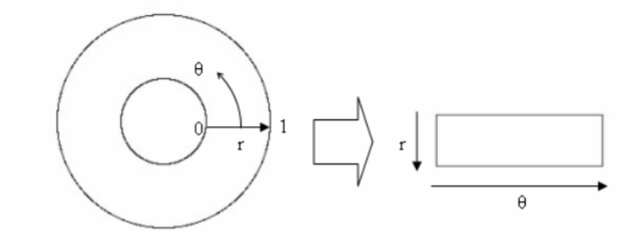
\includegraphics[width=0.90\textwidth]{img/daugman.png}
	\end{center}
	\legend{Fonte: \cite{masek2004}}
\end{figure}

O modelo resultante da aplicação do filtro de Daugman contem as informações da íris que serão utilizadas na identificação. A técnica utilizada no presente relatório utilizada a implementação proposta pro Libor Masek \cite{masek2004}, na qual o método de criação de \textit{template} da íris retorna, após a execução, um modelo no qual as técnicas de reconhecimento podem ser aplicadas. O chamado template biométrico codifica as características da imagem da íris. 
 
% ---
% ----------------------------------------------------------